%        File: arfc-beamer.tex
%     Created: Sun May 5 10:00 PM 2013 C
%


%\documentclass[11pt,handout]{beamer}
\documentclass[9pt]{beamer}
\usetheme[white]{Illinois}
\title[Short Title]{Fluoride-Salt-Cooled High-Temperature Reactor Design Optimization with Evolutionary Algorithms \\ Preliminary Exam}
\author[Your Name]{Gwendolyn J.Y. Chee}
\date[09.13.2021]{September 13, 2021}
\institute{
Dept. of Nuclear, Plasma and Radiological Engineering \\ University of Illinois at Urbana-Champaign
}

%\usepackage{bbding}
\usepackage{amsfonts}
\usepackage{amsmath}
\usepackage{xspace}
\usepackage{graphicx}
\usepackage{booktabs} % nice rules for tables
\usepackage{microtype} % if using PDF
\usepackage{bigints}
\usepackage{minted}

\newcommand{\Cyclus}{\textsc{Cyclus}\xspace}%
\newcommand{\Cycamore}{\textsc{Cycamore}\xspace}%
\newcommand{\deploy}{\texttt{d3ploy}\xspace}%
\newcommand{\units}[1] {\:\text{#1}}%
\newcommand{\SN}{S$_N$}%{S$_\text{N}$}%{$S_N$}%
\DeclareMathOperator{\erf}{erf}
%I need some complimentary error funcitons... 
\DeclareMathOperator{\erfc}{erfc}
%page numbers
\setbeamertemplate{footline}[page number]
\setbeamertemplate{caption}[numbered]
%Those icons in the references are terrible looking
\setbeamertemplate{bibliography item}[text]

\usepackage{tkz-euclide}
\usepackage{tikz}
\usetikzlibrary{positioning, arrows, decorations, shapes}

\usetikzlibrary{shapes.geometric,arrows}
\tikzstyle{process} = [rectangle, rounded corners, minimum width=3cm, minimum height=1cm,text centered, draw=black, fill=blue!30]
\tikzstyle{object} = [ellipse, rounded corners, minimum width=3cm, minimum height=1cm,text centered, draw=black, fill=green!30]
\tikzstyle{arrow} = [thick,->,>=stealth]

\definecolor{illiniblue}{HTML}{B1C6E2}
\definecolor{illiniorange}{HTML}{f8c2a2}
\usetikzlibrary{shapes.geometric, arrows}
\tikzstyle{oblock} = [rectangle, draw, fill=illiniorange, 
text width=15em, text centered, rounded corners, minimum height=4em]
\tikzstyle{bblock} = [rectangle, draw, fill=illiniblue, 
text width=15em, text centered, rounded corners, minimum height=4em]
\tikzstyle{arrow} = [thick,->,>=stealth]

\definecolor{fhrblue}{HTML}{0000ff}
\definecolor{fhrgrey}{HTML}{808080}
\definecolor{fhrred}{HTML}{f10a0a}
\definecolor{fhrgreen}{HTML}{2f6d39}
\definecolor{fhryellow}{HTML}{fdfe36}

\usepackage{tabularx}
\newcolumntype{b}{>{\hsize=1.0\hsize}X}
\newcolumntype{s}{>{\hsize=.5\hsize}X}
\newcolumntype{m}{>{\hsize=.75\hsize}X}
\newcolumntype{x}{>{\hsize=.25\hsize}X}
\newcolumntype{L}{>{\raggedright\arraybackslash}X}
\newcolumntype{R}{>{\raggedleft\arraybackslash}X}
\def\arraystretch{1}
%%%% Acronym support
\usepackage{multirow}
\usepackage{graphicx}
\usepackage{subcaption}

\usepackage[acronym,toc]{glossaries}
%\newacronym{<++>}{<++>}{<++>}
\newacronym[longplural={metric tons of heavy metal}]{MTHM}{MTHM}{metric ton of heavy metal}
\newacronym{3D CAD}{3D CAD}{three-dimensional Computer-Aided Design}
\newacronym{ABM}{ABM}{agent-based modeling}
\newacronym{ACDIS}{ACDIS}{Program in Arms Control \& Domestic and International Security}
\newacronym{AHTR}{AHTR}{Advanced High Temperature Reactor}
\newacronym{AI}{AI}{Artificial Intelligence}
\newacronym{AM}{AM}{Additive Manufacturing}
\newacronym{AMAFT}{AMAFT}{Additive Manufacturing as an Alternative Fabrication Technique}
\newacronym{ANDRA}{ANDRA}{Agence Nationale pour la gestion des D\'echets RAdioactifs, the French National Agency for Radioactive Waste Management}
\newacronym{ANL}{ANL}{Argonne National Laboratory}
\newacronym{ANS}{ANS}{American Nuclear Society}
\newacronym{API}{API}{application programming interface}
\newacronym{ARE}{ARE}{Aircraft Reactor Experiment}
\newacronym{ARFC}{ARFC}{Advanced Reactors and Fuel Cycles}
\newacronym{ARMA}{ARMA}{Autoregressive Moving Average}
\newacronym{ARCH}{ARCH}{Autoregressive Heteroskedasticity}
\newacronym{ARIMA}{ARIMA}{Auto-Regressive Integrated Moving Averages}
\newacronym{ASME}{ASME}{American Society of Mechanical Engineers}
\newacronym{ATWS}{ATWS}{Anticipated Transient Without Scram}
\newacronym{BDBE}{BDBE}{Beyond Design Basis Event}
\newacronym{BIDS}{BIDS}{Berkeley Institute for Data Science}
\newacronym{BNL}{BNL}{Brookhaven National Laboratory}
\newacronym{CAFCA}{CAFCA}{ Code for Advanced Fuel Cycles Assessment }
\newacronym{CDTN}{CDTN}{Centro de Desenvolvimento da Tecnologia Nuclear}
\newacronym{CFD}{CFD}{Computational Fluid Dynamics}
\newacronym{CEA}{CEA}{Commissariat \`a l'\'Energie Atomique et aux \'Energies Alternatives}
\newacronym{CI}{CI}{continuous integration}
\newacronym{CIEMAT}{CIEMAT}{Centro de Investigaciones Energéticas, Medioambientales y Tecnológicas}
\newacronym{CNEN}{CNEN}{Comiss\~{a}o Nacional de Energia Nuclear}
\newacronym{CNERG}{CNERG}{Computational Nuclear Engineering Research Group}
\newacronym{CNRS}{CNRS}{Le Centre National De La Recherche Scientifique}
\newacronym{COSI}{COSI}{Commelini-Sicard}
\newacronym{COTS}{COTS}{commercial, off-the-shelf}
\newacronym{CSNF}{CSNF}{commercial spent nuclear fuel}
\newacronym{CTAH}{CTAHs}{Coiled Tube Air Heaters}
\newacronym{CUBIT}{CUBIT}{CUBIT Geometry and Mesh Generation Toolkit}
\newacronym{CURIE}{CURIE}{Centralized Used Fuel Resource for Information Exchange}
\newacronym{DAG}{DAG}{directed acyclic graph}
\newacronym{DANESS}{DANESS}{Dynamic Analysis of Nuclear Energy System Strategies}
\newacronym{DBE}{DBE}{Design Basis Event}
\newacronym{DEAP}{DEAP}{Distributed Evolutionary Algorithms in Python}
\newacronym{DESAE}{DESAE}{Dynamic Analysis of Nuclear Energy Systems Strategies}
\newacronym{DHS}{DHS}{Department of Homeland Security}
\newacronym{DNBR}{DNBR}{Departure from nucleate boiling ratio}
\newacronym{DOE}{DOE}{Department of Energy}
\newacronym{dpa}{dpa}{displacements per atom}
\newacronym{DRACS}{DRACS}{Direct Reactor Auxiliary Cooling System}
\newacronym{DRE}{DRE}{dynamic resource exchange}
\newacronym{DSNF}{DSNF}{DOE spent nuclear fuel}
\newacronym{DYMOND}{DYMOND}{Dynamic Model of Nuclear Development }
\newacronym{EBM}{EBM}{electron beam melting}
\newacronym{EBS}{EBS}{Engineered Barrier System}
\newacronym{EDF}{EDF}{Électricité de France}
\newacronym{EDZ}{EDZ}{Excavation Disturbed Zone}
\newacronym{EG}{EG}{Evaluation Group}
\newacronym{EIA}{EIA}{U.S. Energy Information Administration}
\newacronym{EPA}{EPA}{Environmental Protection Agency}
\newacronym{EPR}{EPR}{European Pressurized Reactors}
\newacronym{EP}{EP}{Engineering Physics}
\newacronym{EU}{EU}{European Union}
\newacronym{FCM}{FCM}{fully ceramic microencapsulated}
\newacronym{FCO}{FCO}{Fuel Cycle Options}
\newacronym{FCT}{FCT}{Fuel Cycle Technology}
\newacronym{FEHM}{FEHM}{Finite Element Heat and Mass Transfer}
\newacronym{FEPs}{FEPs}{Features, Events, and Processes}
\newacronym{FHR}{FHR}{Fluoride-Salt-Cooled High-Temperature Reactor}
\newacronym{FLiBe}{FLiBe}{Fluoride-Lithium-Beryllium}
\newacronym{FM}{FM}{ferritic/martensitic}
\newacronym{FP}{FP}{Fission Product}
\newacronym{GA}{GA}{Genetic Algorithm}
\newacronym{GDSE}{GDSE}{Generic Disposal System Environment}
\newacronym{GDSM}{GDSM}{Generic Disposal System Model}
\newacronym{GENIUSv1}{GENIUSv1}{Global Evaluation of Nuclear Infrastructure Utilization Scenarios, Version 1}
\newacronym{GENIUSv2}{GENIUSv2}{Global Evaluation of Nuclear Infrastructure Utilization Scenarios, Version 2}
\newacronym{GENIUS}{GENIUS}{Global Evaluation of Nuclear Infrastructure Utilization Scenarios}
\newacronym{GFR}{GFR}{Gas-Cooled Fast Reactor System}
\newacronym{GHG}{GHG}{Greenhouse Gas}
\newacronym{GPAM}{GPAM}{Generic Performance Assessment Model}
\newacronym{GRSAC}{GRSAC}{Graphite Reactor Severe Accident Code}
\newacronym{GUI}{GUI}{graphical user interface}
\newacronym{HFIR}{HFIR}{High Flux Isotope Reactor}
\newacronym{HLW}{HLW}{high level waste}
\newacronym{HPC}{HPC}{high-performance computing}
\newacronym{HTC}{HTC}{high-throughput computing}
\newacronym{HTGR}{HTGR}{High Temperature Gas-Cooled Reactor}
\newacronym{IAEA}{IAEA}{International Atomic Energy Agency}
\newacronym{IEMA}{IEMA}{Illinois Emergency Mangament Agency}
\newacronym{IHLRWM}{IHLRWM}{International High Level Radioactive Waste Management}
\newacronym{INL}{INL}{Idaho National Laboratory}
\newacronym{IPRR1}{IRP-R1}{Instituto de Pesquisas Radioativas Reator 1}
\newacronym{IRP}{IRP}{Integrated Research Project}
\newacronym{IRSN}{IRSN}{Institute for Radiological Protection and Nuclear Safety}
\newacronym{ISFSI}{ISFSI}{Independent Spent Fuel Storage Installation}
\newacronym{ISRG}{ISRG}{Independent Student Research Group}
\newacronym{JAEA}{JAEA}{Japanese Atomic Energy Agency}
\newacronym{JFNK}{JFNK}{Jacobian-Free Newton Krylov}
\newacronym{LANL}{LANL}{Los Alamos National Laboratory}
\newacronym{LBNL}{LBNL}{Lawrence Berkeley National Laboratory}
\newacronym{LCOE}{LCOE}{levelized cost of electricity}
\newacronym{L-DED}{L-DED}{laser directed energy deposition}
\newacronym{LDRD}{LDRD}{laboratory directed research and development}
\newacronym{LEU}{LEU}{low-enriched uranium}
\newacronym{LFR}{LFR}{Lead-Cooled Fast Reactor}
\newacronym{LLNL}{LLNL}{Lawrence Livermore National Laboratory}
\newacronym{LMFBR}{LMFBR}{Liquid Metal Fast Breeder Reactor}
\newacronym{LOFC}{LOFC}{Loss of Forced Cooling}
\newacronym{LOHS}{LOHS}{Loss of Heat Sink}
\newacronym{LOLA}{LOLA}{Loss of Large Area}
\newacronym{LP}{LP}{linear program}
\newacronym{LPD}{LPD}{Local power density}
\newacronym{LWR}{LWR}{Light Water Reactor}
\newacronym{MAGNOX}{MAGNOX}{Magnesium Alloy Graphie Moderated Gas Cooled Uranium Oxide Reactor}
\newacronym{MA}{MA}{minor actinide}
\newacronym{MCNP}{MCNP}{Monte Carlo N-Particle code}
\newacronym{MILP}{MILP}{mixed-integer linear program}
\newacronym{MIT}{MIT}{Massachusetts Institute of Technology}
\newacronym{MOAB}{MOAB}{Mesh-Oriented datABase}
\newacronym{MOOSE}{MOOSE}{Multiphysics Object-Oriented Simulation Environment}
\newacronym{MOSART}{MOSART}{Molten Salt Actinide Recycler and Transmuter}
\newacronym{MOX}{MOX}{mixed oxide}
\newacronym{MPI}{MPI}{Message Passing Interface}
\newacronym{MSBR}{MSBR}{Molten Salt Breeder Reactor}
\newacronym{MSFR}{MSFR}{Molten Salt Fast Reactor}
\newacronym{MSRE}{MSRE}{Molten Salt Reactor Experiment}
\newacronym{MSR}{MSR}{Molten Salt Reactor}
\newacronym{NAGRA}{NAGRA}{National Cooperative for the Disposal of Radioactive Waste}
\newacronym{NEA}{NEA}{Nuclear Energy Agency}
\newacronym{NEAMS}{NEAMS}{Nuclear Engineering Advanced Modeling and Simulation}
\newacronym{NEUP}{NEUP}{Nuclear Energy University Programs}
\newacronym{NFC}{NFC}{Nuclear Fuel Cycle}
\newacronym{NFCSim}{NFCSim}{Nuclear Fuel Cycle Simulator}
\newacronym{NGNP}{NGNP}{Next Generation Nuclear Plant}
\newacronym{NMR-50}{NMR-50}{Purdue Novel Modular Reactor}
\newacronym{NMWPC}{NMWPC}{Nuclear MW Per Capita}
\newacronym{NNL}{NNL}{National Nuclear Laboratory}
\newacronym{NNSA}{NNSA}{National Nuclear Security Administration}
\newacronym{NPP}{NPP}{Nuclear Power Plant}
\newacronym{NPRE}{NPRE}{Department of Nuclear, Plasma, and Radiological Engineering}
\newacronym{NQA1}{NQA-1}{Nuclear Quality Assurance - 1}
\newacronym{NRC}{NRC}{Nuclear Regulatory Commission}
\newacronym{NSF}{NSF}{National Science Foundation}
\newacronym{NSSC}{NSSC}{Nuclear Science and Security Consortium}
\newacronym{NUWASTE}{NUWASTE}{Nuclear Waste Assessment System for Technical Evaluation}
\newacronym{NWF}{NWF}{Nuclear Waste Fund}
\newacronym{NWTRB}{NWTRB}{Nuclear Waste Technical Review Board}
\newacronym{OCRWM}{OCRWM}{Office of Civilian Radioactive Waste Management}
\newacronym{OECD}{OECD}{Organisation for Economic Co-operation and Development}
\newacronym{ORION}{ORION}{ORION}
\newacronym{ORNL}{ORNL}{Oak Ridge National Laboratory}
\newacronym{PARCS}{PARCS}{Purdue Advanced Reactor Core Simulator}
\newacronym{PCA}{PCA}{Particle Collision Algorithm}
\newacronym{PBAHTR}{PB-AHTR}{Pebble Bed Advanced High Temperature Reactor}
\newacronym{PBFHR}{PB-FHR}{Pebble-Bed Fluoride-Salt-Cooled High-Temperature Reactor}
\newacronym{PEI}{PEI}{Peak Environmental Impact}
\newacronym{PH}{PRONGHORN}{PRONGHORN}
\newacronym{PIRT}{PIRT}{Phenomena Identification and Ranking Table}
\newacronym{PPF}{PPF}{Power peaking factor}
\newacronym{PRIS}{PRIS}{Power Reactor Information System}
\newacronym{PRKE}{PRKE}{Point Reactor Kinetics Equations}
\newacronym{PSPG}{PSPG}{Pressure-Stabilizing/Petrov-Galerkin}
\newacronym{PWAR}{PWAR}{Pratt and Whitney Aircraft Reactor}
\newacronym{PWR}{PWR}{Pressurized Water Reactor}
\newacronym{PyNE}{PyNE}{Python toolkit for Nuclear Engineering}
\newacronym{PyRK}{PyRK}{Python for Reactor Kinetics}
\newacronym{QA}{QA}{quality assurance}
\newacronym{RDD}{RD\&D}{Research Development and Demonstration}
\newacronym{RD}{R\&D}{Research and Development}
\newacronym{REE}{REE}{rare earth element}
\newacronym{RELAP}{RELAP}{Reactor Excursion and Leak Analysis Program}
\newacronym{RIA}{RIA}{Reactivity Insertion Accident}
\newacronym{RIF}{RIF}{Region-Institution-Facility}
\newacronym{SA}{SA}{Sensitivity Analysis}
\newacronym{SCK CEN}{SCK CEN}{Studiecentrum voor Kernenergie}
\newacronym{SCWR}{SCWR}{Supercritical-Water-Cooled Reactor System}
\newacronym{SFR}{SFR}{Sodium-Cooled Fast Reactor}
\newacronym{SF-TMSR}{SF-TMSR}{Solid Fuel Thorium Molten Salt Reactor}
\newacronym{SiC}{SiC}{silicon carbide}
\newacronym{SINAP}{SINAP}{Shanghai Institute of Applied Physics}
\newacronym{SINDAG}{SINDA{\textbackslash}G}{Systems Improved Numerical Differencing Analyzer $\backslash$ Gaski}
\newacronym{SKB}{SKB}{Svensk K\"{a}rnbr\"{a}nslehantering AB}
\newacronym{SLM}{SLM}{selective laser melting}
\newacronym{SmAHTR}{SmAHTR}{Small Modular AHTR}
\newacronym{SNF}{SNF}{spent nuclear fuel}
\newacronym{SNL}{SNL}{Sandia National Laboratory}
\newacronym{SLM}{SLM}{selective laser melting}
\newacronym{STC}{STC}{specific temperature change}
\newacronym{SUPG}{SUPG}{Streamline-Upwind/Petrov-Galerkin}
\newacronym{SWF}{SWF}{Separations and Waste Forms}
\newacronym{SWU}{SWU}{Separative Work Unit}
\newacronym{TCR}{TCR}{Transformational Challenge Reactor}
\newacronym{TRIGA}{TRIGA}{Training Research Isotope General Atomic}
\newacronym{TRISO}{TRISO}{Tristructural Isotropic}
\newacronym{TSM}{TSM}{Total System Model}
\newacronym{TSPA}{TSPA}{Total System Performance Assessment for the Yucca Mountain License Application}
\newacronym{ThOX}{ThOX}{thorium oxide}
\newacronym{UFD}{UFD}{Used Fuel Disposition}
\newacronym{UML}{UML}{Unified Modeling Language}
\newacronym{UOX}{UOX}{uranium oxide}
\newacronym{UQ}{UQ}{uncertainty quantification}
\newacronym{US}{US}{United States}
\newacronym{USC}{USC}{University of South Carolina}
\newacronym{UIUC}{UIUC}{University of Illinois at Urbana-Champaign}
\newacronym{UT Austin}{UT Austin}{The University of Texas at Austin}
\newacronym{UW}{UW}{University of Wisconsin}
\newacronym{VISION}{VISION}{the Verifiable Fuel Cycle Simulation Model}
\newacronym{VHTR}{VHTR}{Very-High-Temperature Reactor System}
\newacronym{VVER}{VVER}{Voda-Vodyanoi Energetichesky Reaktor (Russian Pressurized Water Reactor)}
\newacronym{VV}{V\&V}{verification and validation}
\newacronym{YMR}{YMR}{Yucca Mountain Repository Site}


\makeglossaries
\setbeamerfont{subsection in toc}{size=\scriptsize}

%try to get rid of header on title page\dots
\makeatletter
    \newenvironment{withoutheadline}{
        \setbeamertemplate{headline}[default]
        \def\beamer@entrycode{\vspace*{-\headheight}}
    }{}
\makeatother

% add slide numbers
\makeatother
\setbeamertemplate{footline}
{
  \leavevmode%
  \hbox{%
    \rightline{\insertframenumber{} / \inserttotalframenumber\hspace*{1ex}}
  }%
  \vskip0pt%
}
\makeatletter

\begin{document}
%%%%%%%%%%%%%%%%%%%%%%%%%%%%%%%%%%%%%%%%%%%%%%%%%%%%%%%%%%%%%
%% From uw-beamer Here's a handy bit of code to place at 
%% the beginning of your presentation (after \begin{document}):
\newcommand*{\alphabet}{ABCDEFGHIJKLMNOPQRSTUVWXYZabcdefghijklmnopqrstuvwxyz}
\newlength{\highlightheight}
\newlength{\highlightdepth}
\newlength{\highlightmargin}
\setlength{\highlightmargin}{2pt}
\settoheight{\highlightheight}{\alphabet}
\settodepth{\highlightdepth}{\alphabet}
\addtolength{\highlightheight}{\highlightmargin}
\addtolength{\highlightdepth}{\highlightmargin}
\addtolength{\highlightheight}{\highlightdepth}
\newcommand*{\Highlight}{\rlap{\textcolor{HighlightBackground}{\rule[-\highlightdepth]{\linewidth}{\highlightheight}}}}
%%%%%%%%%%%%%%%%%%%%%%%%%%%%%%%%%%%%%%%%%%%%%%%%%%%%%%%%%%%%%
%%--------------------------------%%
\begin{withoutheadline}
\frame{
  \titlepage
}
\end{withoutheadline}

%%--------------------------------%%
\AtBeginSection[]{
\begin{frame}
  \frametitle{Outline}
  \tableofcontents[currentsection]
\end{frame}
}

\section{Introduction}
\subsection{Motivation: AHTR Model Development}
\begin{frame}
    \frametitle{Motivation}
    \begin{itemize}
      \item Energy use and production contribute two-thirds of total \gls{GHG} emissions \cite{noauthor_climate_2018}
      \item Because energy generation technology selection profoundly impacts climate change, 
      large scale emissions-free nuclear power deployment could 
      significantly reduce GHG production but faces both cost and perceived adverse 
      safety challenges \cite{noauthor_climate_2018, petti_future_2018}.
      \item The Generation IV International Forum identified six Generation IV systems 
      that target goals in four areas: sustainability, 
      economics, safety and reliability, and proliferation resistance and physical 
      protection: GFR, LFR, MSR, SFR, SCWR, and VHTR. 
      \begin{figure}[htbp!]
          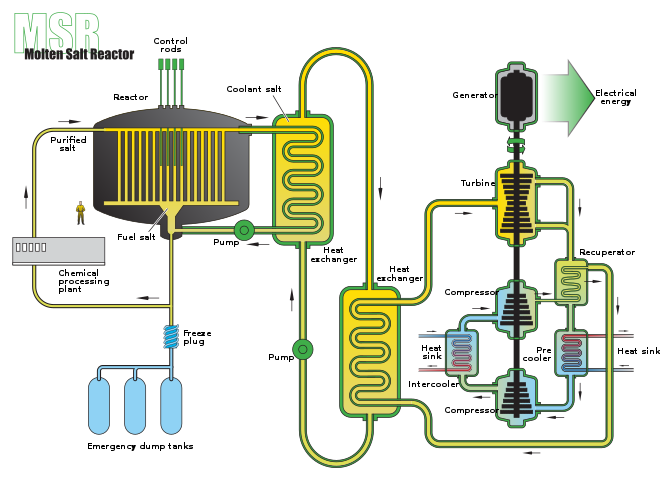
\includegraphics[height=2.8cm]{figures/msr}
          \hspace{1cm}
          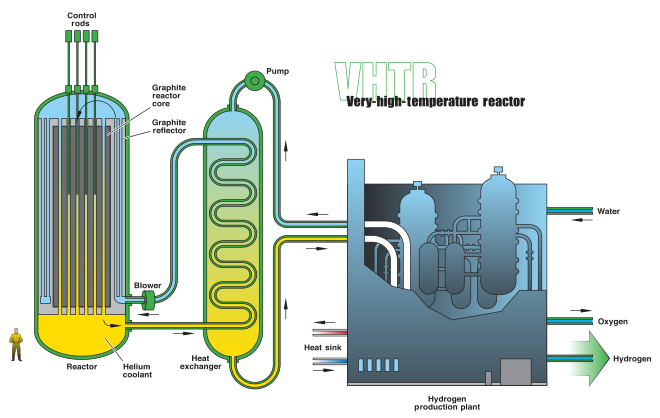
\includegraphics[height=2.8cm]{figures/vhtr}
      \end{figure}
    \end{itemize}
  \end{frame}
\begin{frame}
  \frametitle{Motivation}
  \begin{block}{Molten Salt Reactor (MSR) System}
    \begin{itemize}
      \item Produces fission power in circulating molten salt fuel mixture
      \item Molten Fluoride Salts have have chemical stability, low vapor pressure 
      at high temperatures, good heat transfer properties, resistance against 
      radiation damage, and inert to common structural materials
      \item Inherent system safety with fail-safe drainage, passive cooling, and 
      low inventory of volatile fission products in the fuel
    \end{itemize}
  \end{block}
  \begin{block}{Very High Temperature Reactor System (VHTR)}
    \begin{itemize}
      \item Tristructural Isotropic (TRISO) fuel withstands high burnup and 
      temperature
      \item High outlet temperature increases power conversion efficiency, reduces 
      waste heat generation, and enables high-temperature heat applications 
      such as hydrogen production
      \item Helium coolant's high 100 atm pressurization requires an expensive thick
      concrete reactor vessel
    \end{itemize}
  \end{block}
\end{frame}
\begin{frame}
  \frametitle{Motivation}
  \begin{itemize}
    \item \acrlong{FHR} concept combines the best aspects of \acrlong{MSR} and \acrlong{VHTR} technologies. 
      \acrshort{FHR} use high-temperature coated-particle fuel (similar to the \acrshortpl{VHTR}) 
      and a low-pressure liquid fluoride-salt coolant (similar to the \acrshortpl{MSR})
      \cite{forsberg_fluoride-salt-cooled_2012,facilitators_fluoride-salt-cooled_2013}.
  \end{itemize}
  \begin{block}{\acrfull{FHR} Benefits}
    \begin{itemize}
      \item FHR system has low operating pressure, thus does not require thick 
      concrete pressure vessel 
      \item Molten salt coolant has superior cooling and moderating properties 
      compared to helium coolant in VHTRs
      \item FHR system has large thermal margin enabled by molten salt coolant
      \item FHRs' TRISO particles' solid fuel cladding adds an extra barrier to 
      fission product release compared to MSRs with liquid fuel.
    \end{itemize}
  \end{block}
\end{frame}
\begin{frame}
  \frametitle{Motivation}
  \begin{block}{Advanced High Temperature Reactor Design}
    \begin{itemize}
      \item Design developed by Oak Ridge National Laboratory (ORNL)
      \item Prismatic FHR design with 252 hexagonal fuel assemblies consisting of 
      18 fuel planks arranged in 3 diamond-shaped sectors. 
    \end{itemize}
  \end{block}
  \begin{figure}[]
    \centering
    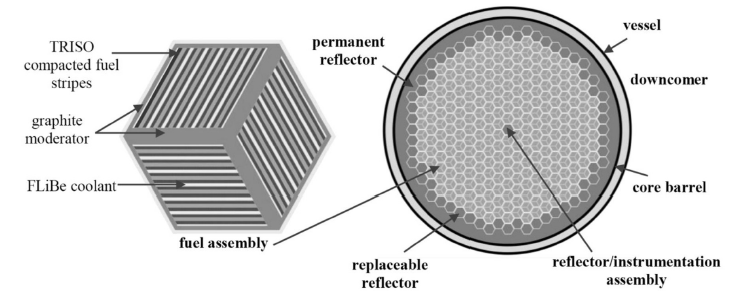
\includegraphics[width=0.8\linewidth]{../docs/figures/ahtr.png} 
    \caption{\acrlong{AHTR} fuel assembly (left) and core configuration (right) 
    reproduced from \cite{ramey_monte_2018}.}
    \label{fig:ahtr}
\end{figure}
\end{frame}

\begin{frame}
  \frametitle{Motivation}
  \begin{block}{Advanced High Temperature Reactor Design}
    \begin{itemize}
      \item Each fuel plank contains 2 fuel stripes that consists of a cubic 
      lattice of TRISO fuel particles
    \end{itemize}
  \end{block}
  \begin{figure}[]
    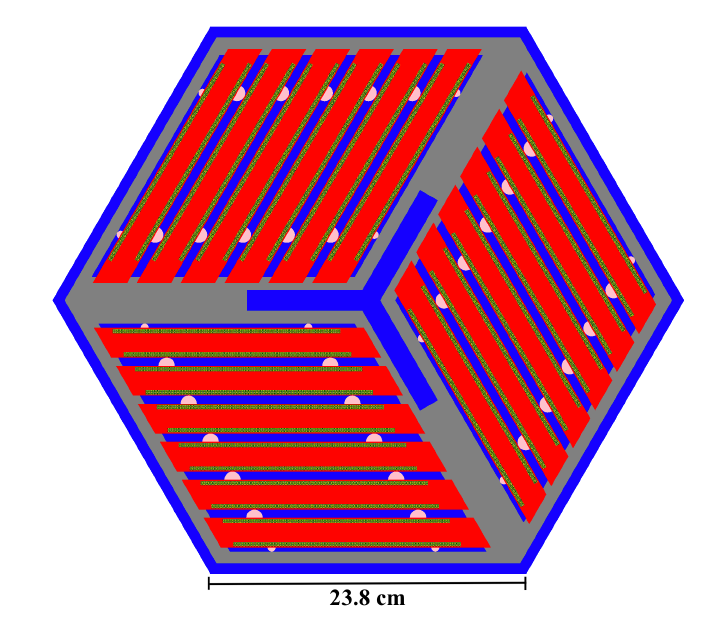
\includegraphics[width=0.5\linewidth]{figures/ahtr-assembly.png} 
    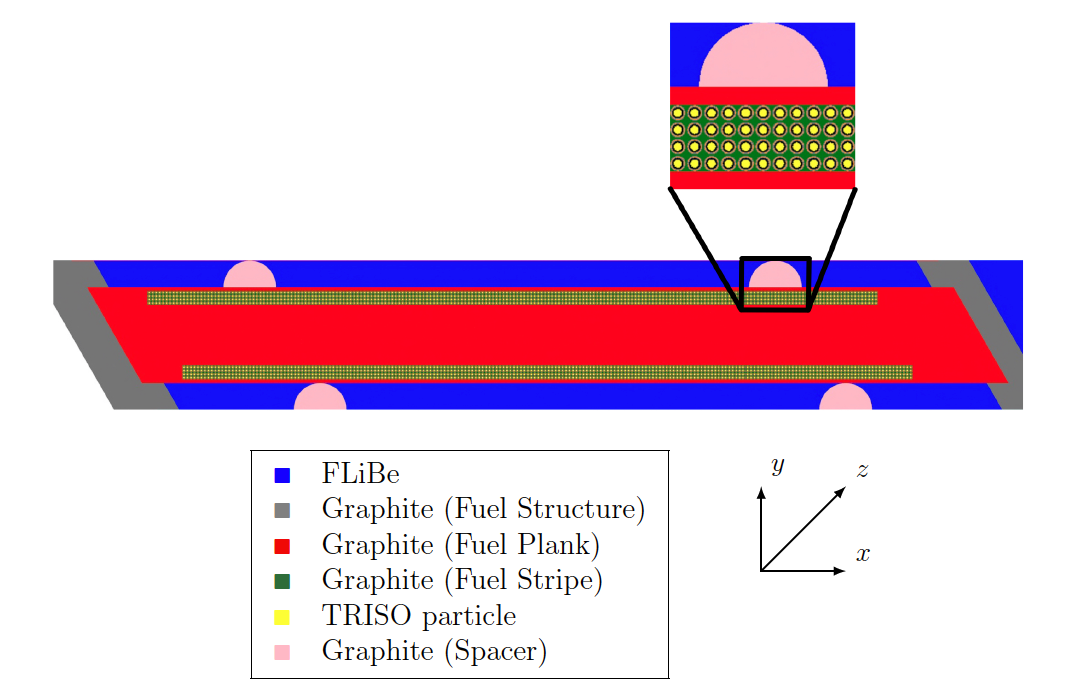
\includegraphics[width=0.5\linewidth]{figures/ahtr-plank.png} 
    \caption{\acrfull{AHTR} fuel assembly with 18 fuel plates arranged in 
    three diamond-shaped sectors, with a central Y-shaped and external channel 
    graphite structure.}
\end{figure}
\end{frame}

\begin{frame}
  \frametitle{Motivation}
  \begin{itemize}
    \item The AHTR's fuel geometry has triple heterogeneity resulting in
    complex reactor physics and significant modeling challenges
    \item To address and further understand the technical challenges for 
    AHTR modeling, in 2019 the OECD-NEA initiated a FHR benchmark exercise. Its objective 
    is to identify the applicability, accuracy, and practicality of the latest 
    methods and codes to assess the current state of the art of FHR simulation 
    and modeling. The benchmark also enables the cross-verification of software 
    and methods for the challenging AHTR geometry, which is especially useful 
    since applicable reactor physics experiments for code validation are scarce
  \end{itemize}
  \begin{figure}[]
    
\includegraphics[width=0.7\linewidth]{figures/benchmark.png} 
    \caption{FHR Benchmark cite.}
\end{figure}
\end{frame}


\subsection{Objectives: AHTR Model Development}
\begin{frame}
  \frametitle{Research Objectives}
  \begin{block}{Technical Gap}
    \begin{itemize}
      \item The triple heterogeneity introduced by the geometrically complex 
      fuel assembly design makes accurate reactor physics simulations challenging. 
      Thus requiring a need to access accuracy of such analyses 
    \end{itemize}
  \end{block}
  \begin{block}{Proposed Work Component I: AHTR Model Development}
    \begin{itemize}
      \item I aim to further our understanding of the AHTR design's complexities 
      through neutronics and thermal-hydraulics modeling.
      \item I will participate in the OECD-NEA's FHR Benchmarking exercise with 
      OpenMC and Moltres
      \item Objectives 
      \begin{itemize}
        \item AHTR 2D and 3D assembly neutronics steady state and depletion models 
        with neutron transport software, OpenMC
        \item AHTR 2D fuel plank and assembly neutronics with thermal hydraulics 
        feedback using Moltres
      \end{itemize}
    \end{itemize}
  \end{block}
\end{frame}

\subsection{Motivation: AHTR Optimization}
\begin{frame}
    \frametitle{3D Printing a Nuclear Reactor?}
    \begin{block}{Impact of Additive Manufacturing Technology Advancements on 
        Reactor Design Optimization}
        \begin{itemize}
            \item With further advancement of additive manufacturing technologies, a reactor 
            core could be 3D printed in the near future
            \item Leveraging additive manufacturing enables us to surpass classical 
            manufacturing constraints and optimize for arbitrary geometries and parameters 
            such as non-uniform channel shapes, and inhomogeneous fuel distribution 
            throughout the core
          \end{itemize}
    \end{block}
    \begin{figure}[]
      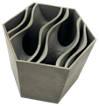
\includegraphics[width=0.2\linewidth]{figures/wavy-channels.png}
      \caption{Example of future reactor design with additively manufactured wavy 
      flow channels}
  \end{figure}
  \end{frame}

  \begin{frame}
    \frametitle{Evolutionary Algorithm Optimization}
    \begin{block}{Evolutionary Algorithms for Reactor Design Optimization}
    \begin{minipage}[c]{0.6\textwidth}
        \begin{itemize}
            \item We can leverage evolutionary algorithm optimization to 
            explore the large design space enabled by 3D printing to find global 
            optimal designs
            \item Evolutionary algorithms have proven successful in optimizing 
            multi-objective problems as they can find solutions at the global 
            optimum and take advantage of parallel systems
            \item Evolutionary algorithms imitate natural selection to evolve solutions 
            \end{itemize}
  \end{minipage}\hfill
  \begin{minipage}[c]{0.4\textwidth}
    \centering
    \begin{figure}
      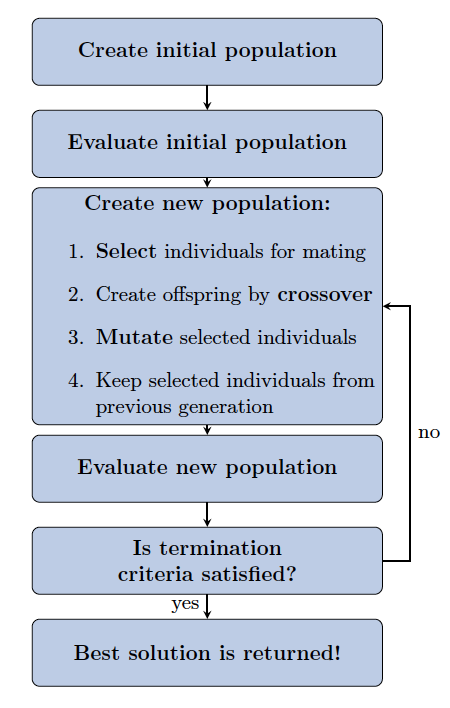
\includegraphics[width=0.8\linewidth]{figures/ea-flow.png} 
      \caption{Evolutionary algorithm flow \cite{renner_genetic_2003}. }
    \end{figure}
  \end{minipage}
  \end{block}
  \end{frame}
    

\subsection{Objectives: AHTR Optimization}
\begin{frame}
    \frametitle{Research Objectives}
    \begin{block}{Technical Gap}
      \begin{itemize}
        \item Applying evolutionary algorithms to nuclear design problems is not new,
        however, evolutionary algorithm setup is highly customizable, A reactor 
        designer unfamiliar with evolutionary algorithms will have to go through 
        the cumbersome process of customizing a genetic algorithm for their
        needs and determine which operators and hyperparameters work best for their problem
      \end{itemize}
    \end{block}
    \begin{block}{Proposed Work Component II: Develop and demonstrate an evolutionary 
        algorithm optimization tool for multi-objective AHTR optimization of 
        non-conventional geometries and fuel distribution}
      \begin{itemize}
        \item Objectives
        \begin{itemize}
            \item Develop a tool that applies evolutionary algorithms with established 
            neutron transport and thermal hydraulics software to optimize reactor 
            design. The tool must be open-source, reproducible, effective, usable,
            and supports HPC parallelization. 
            \item Demonstrate successful implementation of the optimization tool 
            with OpenMC for single and multi-objective AHTR optimization
        \end{itemize}
        \end{itemize}
    \end{block}
  \end{frame}

%\section{Background}
%\subsection{Fluoride-Salt-Cooled High-Temperature Reactor}
%\input{bg_fhr}
%\subsection{Additive Manufacturing}
%\input{bg_am}
%\subsection{Nuclear Reactor Design Optimization}
%\input{bg_opt}
%\subsection{Evolutionary Algorithms}
%\input{bg_ea}
%\subsection{Background Summary}
%\input{bg_summary}

%\section{Fluoride-Salt-Cooled High-Temperature Reactor Benchmark}
%\subsection{Benchmark Description}
%\input{bm_descr}
%\subsection{FHR Benchmark Advanced High Temperature Reactor Design}
%\input{bm_ahtr}
%\subsection{Benchmark Phase I Results}
%\input{bm_phase1}

%\section{Reactor evOLutionary aLgorithm Optimizer (ROLLO)}
%\subsection{ROLLO objectives}
%\input{rollo_obj}
%\subsection{Evolutionary Algorithm Driver}
%\input{rollo_ea}
%\subsection{ROLLO Input File}
%\input{rollo_input}
%\subsection{ROLLO Software Architecture}
%\input{rollo_sw}

%\section{AHTR Optimization Preliminary Work}
%\subsection{ROLLO Optimization: AHTR Fuel Slab}
%\input{prelim_opt}
%\subsection{AHTR Multiphysics Model Preliminary Work}
%\input{prelim_multiphysics}

%\section{Future Work and Proposed Simulations}
%\subsection{AHTR Model Development}
%\input{future_ahtr}
%\subsection{ROLLO Optimization}
%\input{future_rollo}
%\subsection{Conclusion}
%\input{future_concl}


%\input{acks}
%%--------------------------------%%
%%--------------------------------%%
\begin{frame}[allowframebreaks]
  \frametitle{References}
  \bibliographystyle{plain}
  {\footnotesize \bibliography{../docs/2021-chee-prelim.bib} }

\end{frame}

%%--------------------------------%%


\end{document}



